\documentclass[11pt]{article}

\usepackage{amssymb}
\usepackage{setspace}
\usepackage{amsmath}
\usepackage[T1]{fontenc}
\usepackage[utf8]{inputenc}
\usepackage{graphicx}
\usepackage[swedish]{babel}
\usepackage{fixltx2e}
\usepackage{subcaption}
\usepackage{placeins}
\usepackage{fancyhdr}
\usepackage{wrapfig}
\usepackage{tikz}
\usepackage{listings}
\usepackage{hyperref}
\usepackage{gensymb}

\newcommand{\dbar}{d\hspace*{-0.08em}\bar{}\hspace*{0.1em}}

\setlength{\intextsep}{5pt}
\setlength{\textfloatsep}{5pt}

\pagestyle{fancy}
\fancyhf{}
\rhead{SI1121}
\chead{\textbf{Värmepumpen}}
\lhead{Termodynamik}


\begin{document}

\begin{titlepage}
	\centering
	{\scshape\LARGE Värmepumpen \par}
	{\scshape En introduktion för laborationsassistenter \par}
	\vspace{4cm}
	{\scshape\Large Termodynamik \\ SI1121\par}
	\vspace{2cm}
	\vfill
% Bottom of the page
	{\large \today\par}
\end{titlepage}

% -------- Section --------
\section{Förberedelsefrågor}

\subsection{Formulate the second law of thermodynamics}

\begin{equation}
    \mathrm{d}S \geq \frac{\dbar Q}{T}
\end{equation}

Ger en riktning på många typer av reaktioner. Detta förklarar varför vissa saker bara sker i en tidsriktning (kaffet kallnar i en kallare omgivning, universums värmedöd).

\subsection{What is the relation between volume, pressure and temperature in a system where both vapor and fluid are present}

Van der Waals equation

\begin{equation}
    \left ( p + a \left ( \frac{n}{V} \right ) \right ) (V - nb) = nRT
\end{equation}


\subsection{Define entropy and enthalpy}

\begin{equation}
    S = k_\text B \ln \Omega
\end{equation}


Om man har ett system som kan anta ett sätt av mikroskopiska konfigurationer (antalet luftpartiklar med någon hastighet) som tillsammans ger en makroskopisk konfiguration (temperatur i en låda). Vissa makroskopiska konfigurationer kan fås genom många olika typer av mikroskopiska konfigurationer (temperaturen 20\degree C kan uppnås på många sätt om man bara tar hänsyn till partiklars hastighet). Om alla de mikroskopiska konfigurationerna har samma sannolikhet, så kommer systemet gå till den makroskopiska konfiguration med flest antal mikroskopiska sätt att nå det. Entropi kan ses som ett mått på varje energikonfigurations sannolikhet där $\Omega$ är antalet mikrotillstånd var ett givet makrotillstånd.

Vid tidspress - prata om hur många sätt ett ägg kan vara i efter det är krossat jämfört med innan.

\begin{equation}
    H = U + pV
\end{equation}

``Min inre energi plus den energi som krävs för att flytta på min omgivning för att göra plats för min volym''.

\section{Introduktion till pumpen}

\begin{itemize}
    \item Värmepump som använder ett kylämne för att pumpa värme från en reservoar till en annan.
    \item Kompressorn pumpar kylämnet som genomgår en fasövergång
    \item Sex stycken temperaturmätare med ratt för att ändra vilken som mäts
    \item Två stycken tryckklockor 
    \item En effektmätare mellan vägguttag och kompressorsladd (Denna måste stå på W och \underline{\textbf{inte}} MAX W)
\end{itemize}

\section{Studentens arbetsuppgifter}

\begin{itemize}
    \item Fyll upp de båda hinkarna med fyra liter vatten
    \item Gör en tabell och mät sex temperaturer, två tryck\footnote{Glöm ej att lägga på en bar då tryckklockorna mäter övertryck}, och en effekt var femte minut i 40 minuter \footnote{Innan någon mätning kan göras så måste kompressorn stå på i 10 minuter}
    \item Med hjälp av mätvärdena, räkna ut `coefficients of performance' ($\epsilon_v, \ \epsilon$ och $\epsilon_C$)
    \item Rita processen i ett Mollierdiagram
\end{itemize}

\section{Resultat och teori}

\subsection{Coefficients of performance}

\begin{equation}
    \epsilon_v = \frac{Q_1}{W} = \frac{c_{\text{v}} m_{\text{v}} \Delta T}{\langle P \rangle t} \sim 1 \text{ till } 2
\end{equation}

Där $c_{\text{v}} = 4.2$ kJ/kg$\cdot$K vattens specifika värmekapacitet, $m_{\text{v}} = 4$ kg vattnets massa, $\Delta T$ är vattnets uppvärmda temperatur ($T_{\text{slut}} -T_{\text{start}}$), $\langle P \rangle$ medelvärdet av effekten, och $t$ är den totala tiden.

\begin{equation}
    \epsilon = \frac{Q_2 + W}{W} = \frac{c_{\text{v}} m_{\text{v}} \Delta T + c_{\text{is}} m_{\text{is}} + \langle P \rangle t}{\langle P \rangle t} \sim 1 \text{ till } 2
\end{equation}

Där $c_{\text{is}} = 333$ kJ/kg är smältentalpin för vatten, och $m_{\text{is}} \approx 1$ kg isens massa.\footnote{Om studenten vispar så halveras ungefär mängden is} Observera att $\epsilon_v = \epsilon$ om inte systemet har några energiförluster.

\begin{equation}
    \epsilon_C = \frac{T_1}{T_1 - T_2} = \frac{\langle T_1 \rangle}{\langle T_1 \rangle - \langle T_2 \rangle} \sim 7 \text{ till } 9
\end{equation}

Där $T_i, \ i = 1, 2$ motsvarar temperatursensorn med samma nummer. $\epsilon_C$ beräknas för att göra en övre uppskattning på hur bra systemet kan vara. De två andra $\epsilon$ kan sedan jämföras med denna som

\begin{equation}
    \frac{\epsilon_v}{\epsilon_C} = \frac{\epsilon}{\epsilon_C} \sim 0.1 \text{ till } 0.3
\end{equation}

\subsection{Mollierdiagram}

Undersök först Figur \ref{Fig: mollier}.

\begin{figure}[h]
\centering
\begin{subfigure}{.5\textwidth}
  \centering
  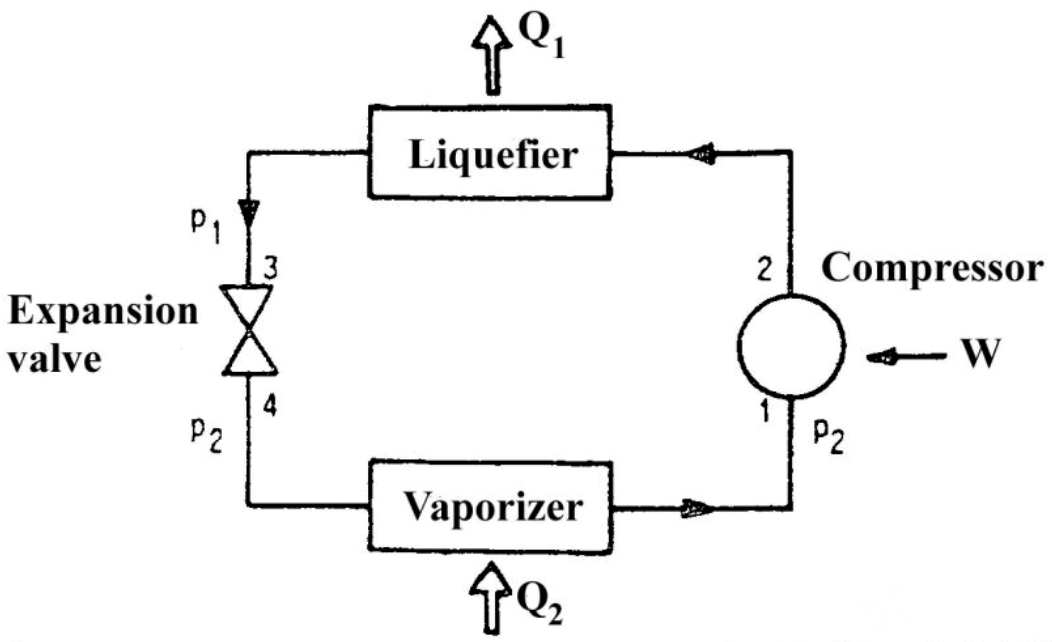
\includegraphics[width=.9\linewidth]{BoxDiagram.png}
  \caption{Boxdiagram över värmepumpen}
\end{subfigure}%
\begin{subfigure}{.5\textwidth}
  \centering
  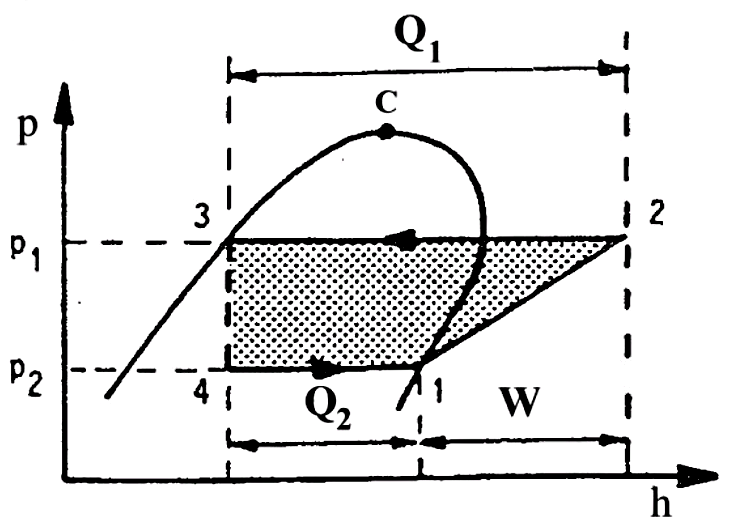
\includegraphics[width=.9\linewidth]{ProcessDiagram.png}
  \caption{Processen ritad i ett Mollierdiagram}
\end{subfigure}
\caption{}
\label{Fig: mollier}
\end{figure}

Där talen 1-4 motsvarar de hörn som grafen har. Genom att känna till vilka temperatursensorer, samt tryckklockor som motsvarar vilket hörn kan processen enkelt ritas ut.

\begin{table}[h]
\centering
\label{my-label}
\begin{tabular}{l|l|l}
Hörn & Temperatursensor & Tryckklocka      \\ \hline
1    & $T_5$            & $p_{\text{blå}}$ \\ \hline
2    & $T_6$            & $p_{\text{röd}}$ \\ \hline
3    & $T_2$            & $p_{\text{röd}}$ \\ \hline
4    & $T_1$            & $p_{\text{blå}}$ \\ \hline
\end{tabular}
\end{table}

Dessa ritas sen ut som $\langle T_i \rangle, \ \langle P_j \rangle$, då det endast är intressant hur processen rör sig ungefär varje varv.

\section{Felkällor}

\begin{itemize}
    \item Uppskattning av mängden is
    \item Osäkerheten i temperatursensorerna (de mäter bara hela \degree C)
\end{itemize}






\end{document}
